\documentclass{sigchi}

% Use this section to set the ACM copyright statement (e.g. for
% preprints).  Consult the conference website for the camera-ready
% copyright statement.

% Copyright
\CopyrightYear{2020}
%\setcopyright{acmcopyright}
\setcopyright{acmlicensed}
%\setcopyright{rightsretained}
%\setcopyright{usgov}
%\setcopyright{usgovmixed}
%\setcopyright{cagov}
%\setcopyright{cagovmixed}
% DOI
\doi{https://doi.org/10.1145/3313831.XXXXXXX}
% ISBN
\isbn{978-1-4503-6708-0/20/04}
%Conference
\conferenceinfo{CHI'20,}{April  25--30, 2020, Honolulu, HI, USA}
%Price
\acmPrice{\$15.00}

% Use this command to override the default ACM copyright statement
% (e.g. for preprints).  Consult the conference website for the
% camera-ready copyright statement.

%% HOW TO OVERRIDE THE DEFAULT COPYRIGHT STRIP --
%% Please note you need to make sure the copy for your specific
%% license is used here!
% \toappear{
% Permission to make digital or hard copies of all or part of this work
% for personal or classroom use is granted without fee provided that
% copies are not made or distributed for profit or commercial advantage
% and that copies bear this notice and the full citation on the first
% page. Copyrights for components of this work owned by others than ACM
% must be honored. Abstracting with credit is permitted. To copy
% otherwise, or republish, to post on servers or to redistribute to
% lists, requires prior specific permission and/or a fee. Request
% permissions from \href{mailto:Permissions@acm.org}{Permissions@acm.org}. \\
% \emph{CHI '16},  May 07--12, 2016, San Jose, CA, USA \\
% ACM xxx-x-xxxx-xxxx-x/xx/xx\ldots \$15.00 \\
% DOI: \url{http://dx.doi.org/xx.xxxx/xxxxxxx.xxxxxxx}
% }

% Arabic page numbers for submission.  Remove this line to eliminate
% page numbers for the camera ready copy
% \pagenumbering{arabic}

% Load basic packages
\usepackage{balance}       % to better equalize the last page
\usepackage{graphics}      % for EPS, load graphicx instead 
\usepackage[T1]{fontenc}   % for umlauts and other diaeresis
\usepackage{txfonts}
\usepackage{mathptmx}
\usepackage[pdflang={en-US},pdftex]{hyperref}
\usepackage{color}
\usepackage{booktabs}
\usepackage{textcomp}

% Some optional stuff you might like/need.
\usepackage{microtype}        % Improved Tracking and Kerning
% \usepackage[all]{hypcap}    % Fixes bug in hyperref caption linking
\usepackage{ccicons}          % Cite your images correctly!
% \usepackage[utf8]{inputenc} % for a UTF8 editor only

% If you want to use todo notes, marginpars etc. during creation of
% your draft document, you have to enable the "chi_draft" option for
% the document class. To do this, change the very first line to:
% "\documentclass[chi_draft]{sigchi}". You can then place todo notes
% by using the "\todo{...}"  command. Make sure to disable the draft
% option again before submitting your final document.
\usepackage{todonotes}

% Paper metadata (use plain text, for PDF inclusion and later
% re-using, if desired).  Use \emtpyauthor when submitting for review
% so you remain anonymous.
\def\plaintitle{Data Philippines}
\def\plainauthor{First Author, Second Author, Third Author,
  Fourth Author, Fifth Author, Sixth Author}
\def\emptyauthor{}
\def\plainkeywords{Open government data; information seeking; }
\def\plaingeneralterms{Documentation, Standardization}

% llt: Define a global style for URLs, rather that the default one
\makeatletter
\def\url@leostyle{%
  \@ifundefined{selectfont}{
    \def\UrlFont{\sf}
  }{
    \def\UrlFont{\small\bf\ttfamily}
  }}
\makeatother
\urlstyle{leo}

% To make various LaTeX processors do the right thing with page size.
\def\pprw{8.5in}
\def\pprh{11in}
\special{papersize=\pprw,\pprh}
\setlength{\paperwidth}{\pprw}
\setlength{\paperheight}{\pprh}
\setlength{\pdfpagewidth}{\pprw}
\setlength{\pdfpageheight}{\pprh}

% Make sure hyperref comes last of your loaded packages, to give it a
% fighting chance of not being over-written, since its job is to
% redefine many LaTeX commands.
\definecolor{linkColor}{RGB}{6,125,233}
\hypersetup{%
  pdftitle={\plaintitle},
% Use \plainauthor for final version.
%  pdfauthor={\plainauthor},
  pdfauthor={\emptyauthor},
  pdfkeywords={\plainkeywords},
  pdfdisplaydoctitle=true, % For Accessibility
  bookmarksnumbered,
  pdfstartview={FitH},
  colorlinks,
  citecolor=black,
  filecolor=black,
  linkcolor=black,
  urlcolor=linkColor,
  breaklinks=true,
  hypertexnames=false
}

% create a shortcut to typeset table headings
% \newcommand\tabhead[1]{\small\textbf{#1}}

% End of preamble. Here it comes the document.
\begin{document}

\title{\plaintitle}

\numberofauthors{3}
\author{%
  \alignauthor{Leave Authors Anonymous\\
    \affaddr{for Submission}\\
    \affaddr{City, Country}\\
    \email{e-mail address}}\\
  \alignauthor{Leave Authors Anonymous\\
    \affaddr{for Submission}\\
    \affaddr{City, Country}\\
    \email{e-mail address}}\\
  \alignauthor{Leave Authors Anonymous\\
    \affaddr{for Submission}\\
    \affaddr{City, Country}\\
    \email{e-mail address}}\\
}

\maketitle

\begin{abstract}
As citizens clamor for transparency and accountability from their national governments, we can see a steady increase in published open government data. Despite this increase, the Philippine government is far from achieving universal participation from its citizens since some form of data literacy is necessary to understand the underlying information from data. This study aims to understand the information seeking and sensemaking behavior of ordinary citizens to evaluate the effectivity of available open government data portals in increasing citizen engagement. We conducted a survey to gauge the awareness of the citizens and an experiment to determine the information seeking behavior of ordinary citizens. \textit{[Results]} \textit{[Contribution]}
\end{abstract}


% ACM Classfication

\begin{CCSXML}
<ccs2012>
<concept>
<concept_id>10003120.10003121</concept_id>
<concept_desc>Human-centered computing~Human computer interaction (HCI)</concept_desc>
<concept_significance>500</concept_significance>
</concept>
<concept>
<concept_id>10003120.10003121.10003125.10011752</concept_id>
<concept_desc>Human-centered computing~Haptic devices</concept_desc>
<concept_significance>300</concept_significance>
</concept>
<concept>
<concept_id>10003120.10003121.10003122.10003334</concept_id>
<concept_desc>Human-centered computing~User studies</concept_desc>
<concept_significance>100</concept_significance>
</concept>
</ccs2012>
\end{CCSXML}

\ccsdesc[500]{Human-centered computing~Human computer interaction (HCI)}
\ccsdesc[300]{Human-centered computing~Haptic devices}
\ccsdesc[100]{Human-centered computing~User studies}

% Author Keywords
\keywords{\plainkeywords}

% Print the classficiation codes
\printccsdesc
Please use the 2012 Classifiers and see this link to embed them in the text: \url{https://dl.acm.org/ccs/ccs_flat.cfm}

\section{Introduction}
The term "\textit{open government}" was first used in the 1950s and was generally used to refer to making previously confidential government information public with the goal of having a government be more politically transparent \cite{YuRobinson2012}. With the advancement of technology and the internet, governments started to launch open government data (OGD) portals as part of their involvement in open government initiatives such as Open Government Partnership \cite{DAWES201615, YuRobinson2012}.

By definition, \textit{open data} should be free to use, share, modify and analyze in machine-readable formats by anyone, but most especially the country's citizens \cite{corrales2019knowledge, DAWES201615}. Open data is perceived to be a useful tool for citizens to demand a more open and collaborative government \cite{warwick2017}. However, despite the initiative of the United Nations to provide guidelines for transparency and citizen engagement \cite{UN2013}, a gap still exists in utilizing OGD for such. It has been argued that most OGD users are technically skilled in analyzing data in its raw formats \cite{DAWES201615}. 

Open Data Philippines (ODPH)\footnote{\url{https://data.gov.ph/}} was launched in January 2014 in fulfilment to the commitments of the Philippines to provide open data \cite{ODPH2015}. Despite the extensive usage of civil society organizations and the private sector, OGD in the Philippines still suffers from low utilization which suggests a disconnect between the published data and the information needs of the citizens \cite{galindesZaplan2018}. 

In governments that have embraced the benefits of OGD, there have been numerous data exploration applications developed through the years. In New York City, the Department of City Planning have different supplementary planning tools that utilize the data that the city has\footnote{\url{https://labs.planning.nyc.gov/projects/}}. In the UK, an open source web tool called Data:In Place\footnote{\url{https://data-in.place/}} was developed to help citizens utilize and understand open government data \cite{puussaar2018making}. Even in other developing countries around the globe, various case studies have been conducted to showcase the potential of open data in these countries \cite{farahi2018}. Although the impact was not quantified, it is suggested that further research may be done to evaluate the effects of OGD in developing countries \cite{farahi2018}.

These tools are examples of what can be done to bridge the gap in citizen engagement with OGD. However, it is necessary first to understand how ordinary citizens interact with data. Given the opportunity for human-computer interaction (HCI) to contribute to this, specifically in the context of a developing country like the Philippines, we are hoping to answer the following research questions:
\begin{itemize}
    \item RQ1: Do open government data portals support t
    \item RQ2: What aspects of the government are the citizens interested in?
    \item RQ3: Where and how do citizens look for information about the government?
    \item RQ4: How effective are Open Data Philippines and Freedom of Information portals in supporting the information seeking and sensemaking needs of the citizens?
\end{itemize}

To answer the first two research questions, we conducted a survey to explore the awareness and interest of Filipino citizens with regard to open government data. To answer the third and fourth research questions, we conducted semi-structured interviews with 21 individuals to observe their information seeking and sensemaking behavior through predetermined tasks. Participants were recruited based on convenience but priority was given to ordinary citizens with little to no experience on data analysis.

We found that ...

This study serves as our formative research in developing a web support tool to better communicate open government data to Filipino citizens.


\section{Related Work}
A survey of research in open government data implementation and human-data interaction (HDI) suggest the need for insights from ordinary citizens since they are also the target users of OGD portals \cite{warwick2017}. While existing HCI and HDI research provide ways of improving OGD portals for experienced data users, understanding behavior of ordinary citizens in contrast with data users present an opportunity to better design OGD portals and other supplementary tools. 

\subsection{OGD Portal Evaluation}
Most research conducted around OGD portals focused on implementation of developed countries \cite{kacprzak2019characterising, klimek2019dcat, koesten2019collaborative,Parycek2014}. Using the Global Open Data Index (GODI) as a reference, countries that have been evaluated in these studies rank relatively high in the list of the 94 countries (See Table \ref{tab:godi})\cite{godimetric2016}. This index only measures the openness of data published according to guidelines under \textit{Open Definition} \cite{godimetric2016}. 

Kl{\'\i}mek focused on evaluating how open data should be published to promote usability, portability, availability and performance \cite{klimek2019dcat}. It showed the value of having a standardized format in publishing metadata to supplement work on Linked Open Data. Parycek et al. \cite{Parycek2014} evaluated Vienna's OGD implementation through understanding the perspectives from both internal and external stakeholders in terms of the process, requirements and benefits. These evaluations are highly beneficial to the government stakeholders to help in improving the implementation of OGD portals as a whole. Our study is similar to \cite{Parycek2014} in the aspect of understanding the targeted end users, specifically evaluating how ordinary citizens perceive ODG portals.

\begin{table}
    \centering
    \begin{tabular}{c c c}
         \textbf{Rank} & \textbf{Country} & \textbf{GODI Score} \\
         \midrule
         2 & Great Britain & 79\% \\
         2 & Australia & 79\% \\
         5 & Canada & 69\% \\
         11 & United States & 65\% \\
         27 & Czech Republic & 50\% \\
         28 & Austria & 49\% \\ 
        %  58 & Philippines & 30\% \\
    \end{tabular}
    \caption{Global Open Data Index (GODI) ranking of countries evaluated by previous research with the Philippines for reference}
    \label{tab:godi}
\end{table}

\subsection{OGD User Studies}
User studies surrounding OGD portals have been focused on individuals who understand how to use data since these are the main users of current OGD portals \cite{choi2017characteristics,kacprzak2019characterising, koesten2019collaborative, koesten2017trials}. Despite the users' experience working with data, current OGD portals have design and implementation limitations in terms of functionalities for search \cite{kacprzak2019characterising, koesten2017trials} and collaborative work \cite{choi2017characteristics, koesten2019collaborative}.

A suggested framework on how data workers interact with data show that behaviors are dependent on the requirements of the task \cite{koesten2017trials}. Despite the existence of data portals, majority of the participants reported using Google to find data needed \cite{koesten2017trials}. To understand further the information seeking behavior of the users, dataset search queries were analyzed together with crowd sourced queries \cite{kacprzak2019characterising}. These studies serve as our basis for conducting experiments with ordinary citizens as the users of an OGD portal. 

\begin{comment}
Collaborative work using OGD was found to be interdisciplinary in nature \cite{choi2017characteristics}. Even though the focus of our study is not on collaborative data work, it is worth noting that the typical projects that emerge from OGD are statistical analysis and exploratory data tools that allow end users to examine data on their own \cite{choi2017characteristics}. 
\end{comment}

\begin{comment}
We conducted a climate survey to gauge the awareness and the interest of Filipino citizens about open government data. We also conducted a pilot study to evaluate the usability of the Open Data Philippines and Freedom of Information portals through search tasks. The survey was distributed electronically through snowball sampling on July 2019 while the usability interviews were conducted between July to August 2019 around the areas of Metro Manila. We obtained participant consent as per research ethics requirements to be able to conduct this study.
\end{comment}

\section{Climate Survey and Portal Analysis}
% rationale for conducting this first study

\subsection{Participants}
The main purpose of our survey was to get a wide range of responses to have an idea of the awareness and the interest of Filipino citizens about open government data. With this, our only requirement for our respondents was to be a Filipino citizen. We utilized snowball sampling by distributing the survey through various social media platforms across different interest groups to further our reach. We also created a Tagalog version of the survey to serve the non-English speaking citizens of the country. We were able to collect a total of 121 responses, 6 from the Tagalog survey. "We tried to include various domains and professional backgrounds to gain a broad overview and avoid unintended biases."


\begin{comment}
\textbf{Survey demographics}
Woman                60 
Man                  52
Prefer not to say     2

Woman                0.526316
Man                  0.456140
Prefer not to say    0.017544

< 20     7
20s     54
30s     28
40s      7
50s      8
60+     10

< 20    0.061404
20s     0.473684
30s     0.245614
40s     0.061404
50s     0.070175
60+     0.087719

Average age: 32.93859649122807, median: 29.0
min       18.000000
25\%       22.250000
50\%       29.000000
75\%       37.000000
max       67.000000

87 have done some sort of data work (76.32\%)
\end{comment}

\subsection{Methods}
The survey had five sections namely, (1) demographic information, (2) background on data work, (3) information seeking sources, (4) awareness of Open Data Philippines and Freedom of Information portals and (5) interest in government data. We asked respondents to provide their age, gender, educational level, income level and current occupation so that we can associate these socio-economic features to their level of awareness and interest in open government data.

For their experience on data work, we specifically asked if they have done any form of data analysis (1) for their main occupation, (2) as a paid part-time job, (3) as a hobby, (4) as a passion or advocacy, (5) for curiosity, and (6) any other type of work. (Reference p835-choi here) We also asked the type of data analysis work they performed for each to understand the depth of data analysis done.

To get a high level understanding of the information seeking behavior of Filipino citizens, we provided specific scenarios and common sources of information and asked them how likely they would use those sources to make a decision in that scenario. 

For the awareness on Open Data Philippines and Freedom of Information portals, we provided the following choices, (1) I did not know about this, (2) I have heard about it, (3) I am aware and have visited (4) I am fully aware and have used or requested datasets. 

At the very end, we also inquired what specific aspect of government data they were interested in to evaluate the availability of data according to the priorities of the respondents. (This is because this study serves as a formative study for the development of an online visualization platform to showcase the open government data to the public.)

\subsection{Results}


\section{Usability Experiment}

\begin{comment}
Age:
min      19.000000
25\%      20.000000
50\%      23.000000
75\%      34.000000
max      64.000000
mean     31.142857

< 20    0.190476
20s     0.428571
30s     0.142857
40s     0.095238
50s     0.047619
60+     0.095238

< 20    4
20s     9
30s     3
40s     2
50s     1
60+     2

M    14 (66.67\%)
F     7 (33.33\%)

Layperson          11
Data Worker         8
Super Layperson     2

Layperson          0.523810
Data Worker        0.380952
Super Layperson    0.095238

Student                                                     9
Professor                                                   2
Bartender                                                   1
Pedicab Driver and Barangay Official                        1
Revenue Assurance Manager                                   1
Baranggay Kagawad                                           1
Barista at Starbucks,SK chairman in Brgy Sta Mesa Manila    1
Senior Data Engineer                                        1
Barista                                                     1
Baranggay Captain,Textbook Distributor                      1
Barangay Kagawad                                            1
IT Consultant                                               1

	count	mean	std	min	25%	50%	75%	max
CLASSIFICATION								
Data Worker	8.0	31.250000	13.812520	19.0	22.00	29.5	34.00	62.0
Layperson	11.0	27.363636	14.541477	19.0	20.00	21.0	24.00	64.0
Super Layperson	2.0	51.500000	10.606602	44.0	47.75	51.5	55.25	59.0
\end{comment}


\begin{table*}
  \centering
  \begin{tabular}{l p{5.2cm} p{5.2cm}}
    % \toprule
    {\small\textit{Portal}}
    & {\small \textit{Personal Task}}
      & {\small \textit{Impersonal Task}}\\
    \midrule
    Open Search & How prevalent is crime in the province where you live? & Find the number of students enrolled in the University of the Philippines during 2015.\\
    Open Data Philippines & How much, in Philippine Peso,  was lost due to fire in your city of residence in 2013? & What are the top countries that most Philippine presidents go to as part of their work? \\
    Freedom of Information & How many people have work in your region? & How many road accidents happened in Metro Manila in 2018?
    % \bottomrule
  \end{tabular}
  \caption{List of search tasks performed by the participants per portal.}~\label{tab:searchtasks}
\end{table*}

We conducted interviews with a different sample of people to understand better the information seeking and sensemaking behaviors of ordinary citizens. Each participant was asked to perform the same number of search tasks. There were three parts with two tasks per part. Table \ref{tab:searchtasks} shows the specific questions that were asked. 

In the open search, participants were allowed to use their preferred search engine, while in the other two parts, they were restricted to search only within the mentioned portal. Tasks were designed based on the assumption that the information is available in either a dataset from Open Data Philippines or a request in the Freedom of Information portal. The logic behind identifying the participant's place of residence as part of the personal task is based on previous studies that show people associate better with data when it is linked to a place (Cite Data:In Place).

All participants were timed for each task to quantify how long it took for them to complete the task. Each participant was given a 15-minute time limit to complete each task due to the constraint of the screen recording software used. They were also given the option to give up at any point. After each task, participants were asked about their experience and their thought process of how they approached the problem.

We also provided the participants six different datasets downloaded from the two government portals for them to rank their usability and provide the basis for their ranking. The goal of this task is to understand the thought process of ordinary citizens and the factors they consider when presented with raw datasets instead of organized information. 

Participants were also asked about their experience with data analysis to allow for comparison between a lay person and a data worker. To be considered a lay person, the participant needed to (1) have less than a year of experience of data analysis and (2) never utilized open government data portals for any kind of work; otherwise, they would be categorized as a data worker. Due to constraints, our participants were selected out of convenience. We were able to successfully recruit 13 lay people and 8 data workers for our interview.

\subsection{Data Analysis}
Inductive coding - Exploratory in nature
\url{https://medium.com/@projectux/themes-dont-just-emerge-coding-the-qualitative-data-95aff874fdce}

descriptive coding - summarizes the primary topic
process coding - word or phrase that captures the action
in vivo coding - using the participant's own words

structural coding is a question-based code that acts as a labelling and index device, allowing researchers to quickly access data likely to be relevant to a particular analysis from a larger data set. Its used as a categorisation technique for further qualitative data analysis.

We have a mix of quantitative and qualitative data from the survey responses, field notes from the interviews, interview transcripts and screen recordings. For the qualitative data, we used topic coding to categorize the responses according to the research questions.

Understanding the level of awareness of Filipino citizens about Open Data Philippines and Freedom of Information (RQ1) and their interest in open government data (RQ2) required processing and analyzing the responses from the survey which were quantitative in nature because of the Likert-scale responses. For the free form wild card questions on interests not included in the predefined options, we used thematic analysis to group together responses.

To understand the information seeking behavior of Filipinos (RQ3), we took the screen recordings and analyzed the different websites the participants used to find answers to the tasks presented. We also analyzed the search queries used per task to come up with the most common used keywords. In addition, we also analyzed data from the information seeking section of our survey.

Lastly, to evaluate the efficacy of the Open Data Philippines and Freedom of Information portals (RQ4), we analyzed the responses of the interviewees to identify the features that supported and restricted them from completing the tasks. 

\textit{Where do the speed of finding the responses come in?}


\section{Results}

Issue encountered with interview:
- 2 interviewees: first time to use a computer/unfamiliar with searching

\subsection{RQ1: How aware are citizens about open government data and Freedom of Information in the Philippines?}

I did not know about this.                      51
I have heard about it.                          39
I am fully aware and have used its datasets.    12
I am aware and have visited it.                 12

I did not know about this.                      0.447368
I have heard about it.                          0.342105
I am fully aware and have used its datasets.    0.105263
I am aware and have visited it.                 0.105263

I did not know about this.                      61
I have heard about it.                          31
I am aware and have visited it.                 11
I am fully aware and have requested from it.    11

I did not know about this.                      0.535088
I have heard about it.                          0.271930
I am aware and have visited it.                 0.096491
I am fully aware and have requested from it.    0.096491

\subsection{RQ2: What aspects of the government are the citizens interested in?}

\textit{How to rank the categories? We have top 3. We can weight the categories according to 3, 2, 1?}

\subsection{RQ3: Where and how do citizens look for information about the government?}

\subsubsection{Common Sources}
- Information seeking section of survey
- Most common pages visited

\subsubsection{Behavior of the interviewees}

\subsection{RQ4: How effective are Open Data Philippines and Freedom of Information portals in supporting the information seeking and sensemaking needs of the citizens?}


\section{Discussion}
\begin{comment}
From model paper:
We address our frst two research questions by summarizing our results. We then discuss insights to broader policy implications to improve the feasibility of online grocery delivery services within low-income and transportation-scarce regions. We conclude by contributing design implications for how online-grocery service interfaces can address participant barriers to using such services. To answer our fnal research question, we leverage past HCI literature to support our implications and further extend the literature.
\end{comment}


\section{Limitations}
- A more statistical approach for sampling for the survey to get a better representation of the population

\section{Conclusion and Future Work}
Summary of what we did and what we found out

Our contribution

Moving forward, we would like to understand whether our design suggestions facilitate a better way to communicate open government data to the general public, even to those with minimal data literacy. 

\begin{comment}
\section{Typeset Text}
The styles contained in this document have been modified from the
default styles to reflect ACM formatting conventions. For example,
content paragraphs like this one are formatted using the Normal style.

\LaTeX\ sometimes will create overfull lines that extend into columns.
To attempt to combat this, the \texttt{.cls} file has a command,
\texttt{{\textbackslash}sloppy}, that essentially asks \LaTeX\ to
prefer underfull lines with extra whitespace.  For more details on
this, and info on how to control it more finely, check out
{\url{http://www.economics.utoronto.ca/osborne/latex/PMAKEUP.HTM}}.

\subsection{Title and Authors}

Your paper's title, authors and affiliations should run across the
full width of the page in a single column 17.8 cm (7 in.) wide.  The
title should be in Helvetica or Arial 18-point bold.  Authors' names
should be in Times New Roman or Times Roman 12-point bold, and
affiliations in 12-point regular.  

See \texttt{{\textbackslash}author} section of this template for
instructions on how to format the authors. For more than three
authors, you may have to place some address information in a footnote,
or in a named section at the end of your paper. Names may optionally
be placed in a single centered row instead of at the top of each
column. Leave one 10-point line of white space below the last line of
affiliations.

\subsection{Abstract and Keywords}

Every submission should begin with an abstract of about 150 words,
followed by a set of Author Keywords and ACM Classification
Keywords. The abstract and keywords should be placed in the left
column of the first page under the left half of the title. The
abstract should be a concise statement of the problem, approach, and
conclusions of the work described. It should clearly state the paper's
contribution to the field of HCI\@.

\subsection{Normal or Body Text}

Please use a 10-point Times New Roman or Times Roman font or, if this
is unavailable, another proportional font with serifs, as close as
possible in appearance to Times Roman 10-point. Other than Helvetica
or Arial headings, please use sans-serif or non-proportional fonts
only for special purposes, such as source code text.

\subsection{First Page Copyright Notice}
This template include a sample ACM copyright notice at the bottom of
page 1, column 1.  Upon acceptance, you will be provided with the
appropriate copyright statement and unique DOI string for publication.
Accepted papers will be distributed in the conference
publications. They will also be placed in the ACM Digital Library,
where they will remain accessible to thousands of researchers and
practitioners worldwide. See
\url{http://acm.org/publications/policies/copyright_policy} for the
ACM's copyright and permissions policy.

\subsection{Subsequent Pages}

On pages beyond the first, start at the top of the page and continue
in double-column format.  The two columns on the last page should be
of equal length.

\begin{figure}
\centering
  
\includegraphics[width=0.9\columnwidth]{figures/sigchi-logo}
  \caption{Insert a caption below each figure. Do not alter the
    Caption style.  One-line captions should be centered; multi-line
    should be justified. }~\label{fig:figure1}
\end{figure}

\subsection{References and Citations}

Use a numbered list of references at the end of the article, ordered
alphabetically by last name of first author, and referenced by numbers
in
brackets~\cite{acm_categories,ethics,Klemmer:2002:WSC:503376.503378}.
Your references should be published materials accessible to the
public. Internal technical reports may be cited only if they are
easily accessible (i.e., you provide the address for obtaining the
report within your citation) and may be obtained by any reader for a
nominal fee. Proprietary information may not be cited. Private
communications should be acknowledged in the main text, not referenced
(e.g., ``[Borriello, personal communication]'').

References should be in ACM citation format:
\url{http://acm.org/publications/submissions/latex_style}. This
includes citations to internet
resources~\cite{acm_categories,cavender:writing,CHINOSAUR:venue,psy:gangnam}
according to ACM format, although it is often appropriate to include
URLs directly in the text, as above.


% Use a numbered list of references at the end of the article, ordered
% alphabetically by first author, and referenced by numbers in
% brackets~\cite{ethics, Klemmer:2002:WSC:503376.503378,
%   Mather:2000:MUT, Zellweger:2001:FAO:504216.504224}. For papers from
% conference proceedings, include the title of the paper and an
% abbreviated name of the conference (e.g., for Interact 2003
% proceedings, use \textit{Proc. Interact 2003}). Do not include the
% location of the conference or the exact date; do include the page
% numbers if available. See the examples of citations at the end of this
% document. Within this template file, use the \texttt{References} style
% for the text of your citation.

% Your references should be published materials accessible to the
% public.  Internal technical reports may be cited only if they are
% easily accessible (i.e., you provide the address for obtaining the
% report within your citation) and may be obtained by any reader for a
% nominal fee.  Proprietary information may not be cited. Private
% communications should be acknowledged in the main text, not referenced
% (e.g., ``[Robertson, personal communication]'').

\begin{table}
  \centering
  \begin{tabular}{l r r r}
    % \toprule
    & & \multicolumn{2}{c}{\small{\textbf{Test Conditions}}} \\
    \cmidrule(r){3-4}
    {\small\textit{Name}}
    & {\small \textit{First}}
      & {\small \textit{Second}}
    & {\small \textit{Final}} \\
    \midrule
    Marsden & 223.0 & 44 & 432,321 \\
    Nass & 22.2 & 16 & 234,333 \\
    Borriello & 22.9 & 11 & 93,123 \\
    Karat & 34.9 & 2200 & 103,322 \\
    % \bottomrule
  \end{tabular}
  \caption{Table captions should be placed below the table. We
    recommend table lines be 1 point, 25\% black. Minimize use of
    table grid lines.}~\label{tab:table1}
\end{table}

\section{Sections}

The heading of a section should be in Helvetica or Arial 9-point bold,
all in capitals. Sections should \textit{not} be numbered.

\subsection{Subsections}

Headings of subsections should be in Helvetica or Arial 9-point bold
with initial letters capitalized.  For sub-sections and
sub-subsections, a word like \emph{the} or \emph{of} is not
capitalized unless it is the first word of the heading.

\subsubsection{Sub-subsections}

Headings for sub-subsections should be in Helvetica or Arial 9-point
italic with initial letters capitalized.  Standard
\texttt{{\textbackslash}section}, \texttt{{\textbackslash}subsection},
and \texttt{{\textbackslash}subsubsection} commands will work fine in
this template.

\section{Figures/Captions}

Place figures and tables at the top or bottom of the appropriate
column or columns, on the same page as the relevant text (see
Figure~\ref{fig:figure1}). A figure or table may extend across both
columns to a maximum width of 17.78 cm (7 in.).

\begin{figure*}
  \centering
  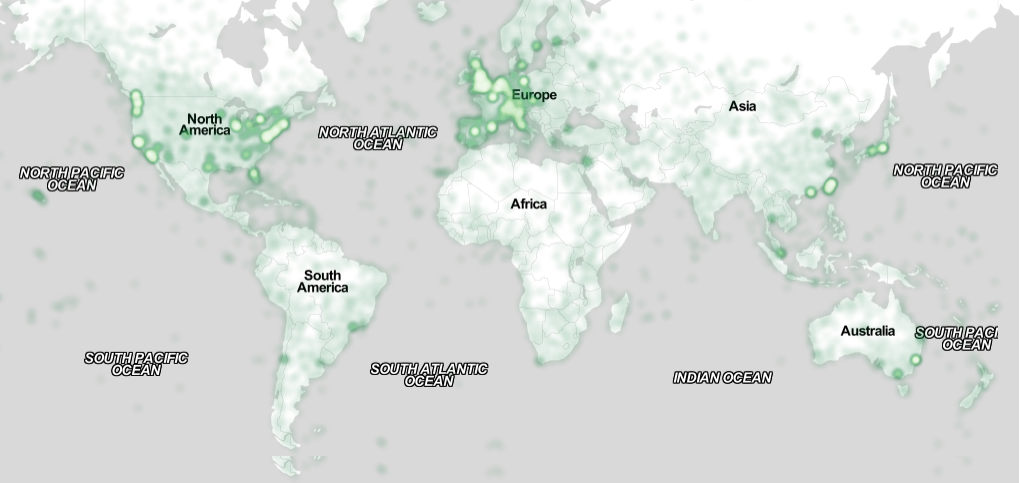
\includegraphics[width=1.75\columnwidth]{figures/map}
  \caption{In this image, the map maximizes use of space. You can make
    figures as wide as you need, up to a maximum of the full width of
    both columns. Note that \LaTeX\ tends to render large figures on a
    dedicated page. Image: \ccbynd~ayman on
    Flickr.}~\label{fig:figure2}
\end{figure*}

Captions should be Times New Roman or Times Roman 9-point bold.  They
should be numbered (e.g., ``Table~\ref{tab:table1}'' or
``Figure~\ref{fig:figure1}''), centered (if one line) otherwise justified, and placed beneath the figure
or table.  Please note that the words ``Figure'' and ``Table'' should
be spelled out (e.g., ``Figure'' rather than ``Fig.'') wherever they
occur. Figures, like Figure~\ref{fig:figure2}, may span columns and
all figures should also include alt text for improved accessibility.
Papers and notes may use color figures, which are included in the page
limit; the figures must be usable when printed in black-and-white in
the proceedings.

The paper may be accompanied by a short video figure (we recommend staying within five
minutes in length). However, the paper should stand on its own without
the video figure, as the video may not be available to everyone who
reads the paper.  

\subsection{Inserting Images}
When possible, include a vector formatted graphic (i.e. PDF or EPS).
When including bitmaps,  use an image editing tool to resize the image
at the appropriate printing resolution (usually 300 dpi).

\section{Quotations}
Quotations may be italicized when \textit{``placed inline''}.

\begin{quote}
Longer quotes, when placed in their own paragraph, need not be
italicized or in quotation marks when indented.  
\end{quote}

\section{Language, Style, and Content}

The written and spoken language of SIGCHI is English. Spelling and
punctuation may use any dialect of English (e.g., British, Canadian,
US, etc.) provided this is done consis- tently. Hyphenation is
optional. To ensure suitability for an international audience, please
pay attention to the following:

\begin{itemize}
\item Write in a straightforward style.
\item Try to avoid long or complex sentence structures.
\item Use common and basic vocabulary (e.g., use the word ``unusual'' rather than the word ``arcane''.
\item Briefly define or explain all technical terms that may be
  unfamiliar to readers.
\item Explain all acronyms the first time they are used in your
  text---e.g., ``Digital Signal Processing (DSP)''.
\item Explain local references (e.g., not everyone knows all city
  names in a particular country).
\item Explain ``insider'' comments. Ensure that your whole audience
  understands any reference whose meaning you do not describe (e.g.,
  do not assume that everyone has used a Macintosh or a particular
  application).
\item Explain colloquial language and puns. Understanding phrases like
  ``red herring'' may require a local knowledge of English.  Humor and
  irony are difficult to translate.
\item Use unambiguous forms for culturally localized concepts, such as
  times, dates, currencies, and numbers (e.g., ``1--5--97'' or
  ``5/1/97'' may mean 5 January or 1 May, and ``seven o'clock'' may
  mean 7:00 am or 19:00). For currencies, indicate equivalences:
  ``Participants were paid {\fontfamily{txr}\selectfont \textwon}
  25,000, or roughly US \$22.''
\item Be careful with the use of gender-specific pronouns (he, she)
  and other gendered words (chairman, manpower, man-months). Use
  inclusive language that is gender-neutral (e.g., she or he, they,
  s/he, chair, staff, staff-hours, person-years). See the
  \textit{Guidelines for Bias-Free Writing} for further advice and
  examples regarding gender and other personal
  attributes~\cite{Schwartz:1995:GBF}. Be particularly aware of
  considerations around writing about people with disabilities.
\item If possible, use the full (extended) alphabetic character set
  for names of persons, institutions, and places (e.g.,
  Gr{\o}nb{\ae}k, Lafreni\'ere, S\'anchez, Nguy{\~{\^{e}}}n,
  Universit{\"a}t, Wei{\ss}enbach, Z{\"u}llighoven, \r{A}rhus, etc.).
  These characters are already included in most versions and variants
  of Times, Helvetica, and Arial fonts.
\end{itemize}

\section{Accessibility}
The Executive Council of SIGCHI has committed to making SIGCHI
conferences more inclusive for researchers, practitioners, and
educators with disabilities. As a part of this goal, the all authors
are asked to work on improving the accessibility of their
submissions. Specifically, we encourage authors to carry out the
following five steps:
\begin{enumerate}
\item Add alternative text to all figures
\item Mark table headings
\item Add tags to the PDF
\item Verify the default language
\item Set the tab order to ``Use Document Structure''
\end{enumerate}
For more information and links to instructions and resources, please
see: \url{http://chi2016.acm.org/accessibility}.  The
\texttt{{\textbackslash}hyperref} package allows you to create well tagged PDF files,
please see the preamble of this template for an example.

\section{Page Numbering, Headers and Footers}
Your final submission should not contain footer or header information
at the top or bottom of each page. Specifically, your final submission
should not include page numbers. Initial submissions may include page
numbers, but these must be removed for camera-ready. Page numbers will
be added to the PDF when the proceedings are assembled.

\section{Producing and Testing PDF Files}

We recommend that you produce a PDF version of your submission well
before the final deadline.  Your PDF file must be ACM DL
Compliant. The requirements for an ACM Compliant PDF are available at:
{\url{http://www.scomminc.com/pp/acmsig/ACM-DL-pdfs-requirements.htm}}.

Test your PDF file by viewing or printing it with the same software we
will use when we receive it, Adobe Acrobat Reader Version 10. This is
widely available at no cost. Note that most
reviewers will use a North American/European version of Acrobat
reader, so please check your PDF accordingly.
\end{comment}


\section{Acknowledgments}

Sample text: We thank all the volunteers, and all publications support
and staff, who wrote and provided helpful comments on previous
versions of this document. Authors 1, 2, and 3 gratefully acknowledge
the grant from NSF (\#1234--2012--ABC). \textit{This whole paragraph is
  just an example.}
  


% Balancing columns in a ref list is a bit of a pain because you
% either use a hack like flushend or balance, or manually insert
% a column break.  http://www.tex.ac.uk/cgi-bin/texfaq2html?label=balance
% multicols doesn't work because we're already in two-column mode,
% and flushend isn't awesome, so I choose balance.  See this
% for more info: http://cs.brown.edu/system/software/latex/doc/balance.pdf
%
% Note that in a perfect world balance wants to be in the first
% column of the last page.
%
% If balance doesn't work for you, you can remove that and
% hard-code a column break into the bbl file right before you
% submit:
%
% http://stackoverflow.com/questions/2149854/how-to-manually-equalize-columns-
% in-an-ieee-paper-if-using-bibtex
%
% Or, just remove \balance and give up on balancing the last page.
%
\balance{}
% BALANCE COLUMNS
\balance{}

% REFERENCES FORMAT
% References must be the same font size as other body text.
\bibliographystyle{SIGCHI-Reference-Format}
\bibliography{sample}

\end{document}

%%% Local Variables:
%%% mode: latex
%%% TeX-master: t
%%% End:
